\section{Analyzing ESBL E. coli isolates from patients
of the University hospital Basel}
\subsection{Sample selection}
The sample collection consisted of 65 samples screened positive for ESBL genes coming from 34 patients. An identifier was created for each sample consisting of the patient number and the sample number. Sample numbers chronologically increased meaning that sample 0 was the first sample collected from a patient. From the 34 patients we had to select for patients wich were suitable for our analysis. Obviously multiple samples per patient were necessary which was not the case for 15 patients. In order that SNPs could be identified which were likely associated with resistance it was necessary that the samples collected from one patient were the same ESBL E. coli strain. By building a phylogenic tree of all the samples we could check how closely related different samples were.  

\subsubsection{Pylogeneic analysis with panX}
\begin{figure}
	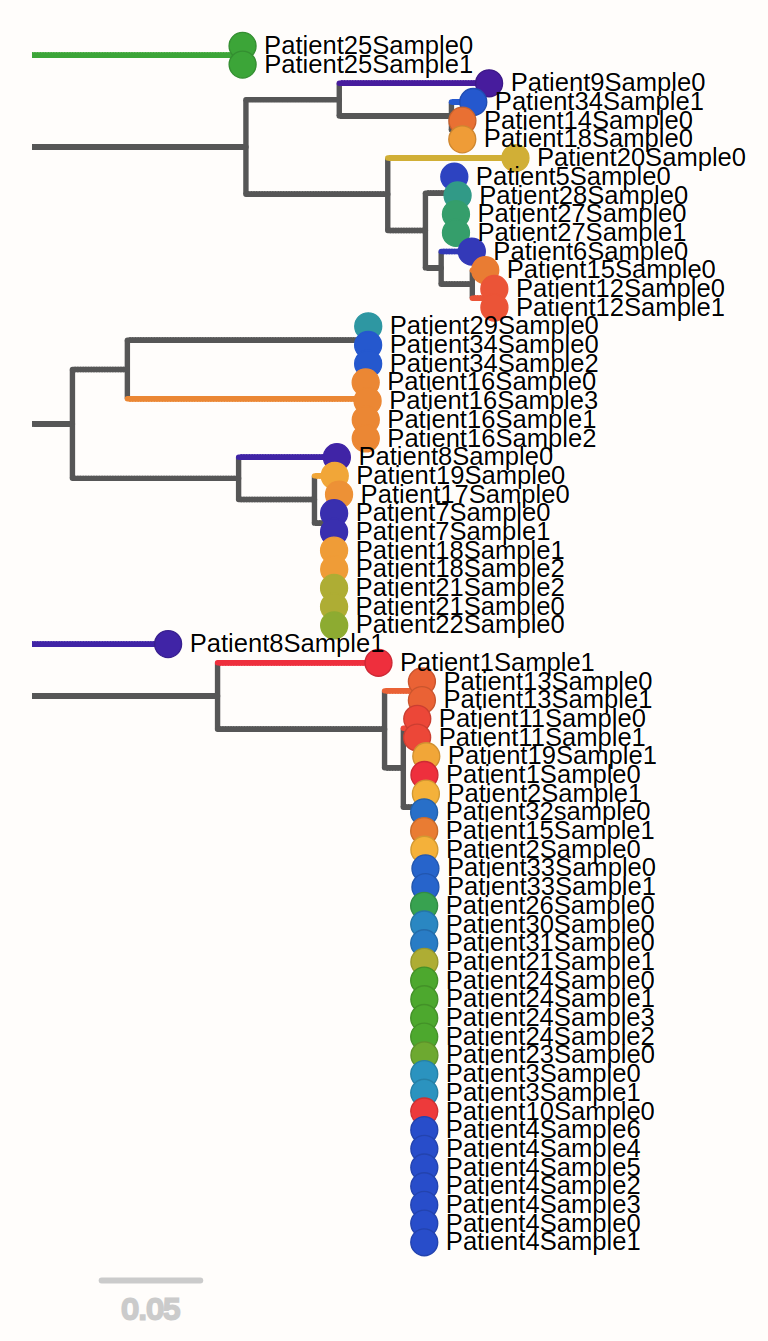
\includegraphics[scale=0.2]{181205_panXtree_overview.png}
	\caption{Phylogenic tree built wihn panX. The samples are colored by the patient.}
	\label{figure:panX}
\end{figure}
Only patients could be used for the analysis where every sample mapped on the same branch on the phylogenetic tree created with PanX. If that was the case the samples shared the identical core genomes. 
Samples of one patient mapping on different branches imply that their core genome differed and they were different strains. Therefore the patient was infected with different strains over the sample period which made it impossible for us to identify SNPs potentially involved in the resistance mechanism. \\
From the 19 patients with multiple samples 7 patients had samples which mapped on different branches. This is visible in Figure \ref{figure:panX}. For example patient 15 had two samples which mapped on two different clades of the tree.
Those 7 patients had to be excluded from the analysis as well. \\
It's also visible in Figure \ref{figure:panX} that some samples from different patients map on the same branch. This tells us, that some patients were infected by the same strain coming probably from the same outbreak within the hospital. On the other hand patient 25 has two samples which map on a separate clade of the pyhlogenic tree. This indicates that this patient most likely got infected outside the hospital.  

What also reduced the patients which could be used for the analysis was that not all of them had a significant increase or decrease of the MIC for cefepime or ceftazidime. Since those MIC were determined by a 2-fold dilution series it was not enough when the concentration doubled over time. This reduced the selection to 5 patients. The meta data and the MIC for those patients are shown in Table \ref{table:samples_overview}. 
\begin{table}
	\begin{tabular}{|c c c c c|}	
		\hline
		Accession & Sample date & MIC Cefepim & MIC Cefepim Sandra & Ceftazidim \\ [0.5ex]
		\hline\hline
		\rowcolor{LightCyan}
		Patient12Sample0 & 9.9.14 & 4 & 16 & 0.75 \\
		Patient12Sample1 & 5.12.14 & 12 & 32 & 2 \\
		\hline
		\rowcolor{LightCyan}
		Patient16Sample0 & 22.6.12 & 8 & 32 & 2\\
		Patient16Sample1 & 18.7.13 & 48 & 64 & 8\\
		Patient16Sample2 & 1.11.13 & 32 & 32 & 12\\
		\hline
		\rowcolor{LightCyan}
		Patient24Sample0 & 02.05.11 & 4 & 16 & 1.5\\
		Patient24Sample1 & 08.15.11 & 16 & 32 & 1.5\\
		Patient24Sample2 & 11.28.11 & 3 & 8 & 1\\
		\hline
		Patient25Sample0 & 15.4.11 & 64 & None & 192\\
		\rowcolor{LightCyan}
		Patient25Sample1 & 22.8.11 & 6 & 4 & 6\\
		\hline
		Patient33Sample0 & 26.9.14 & 24 & None & 16 \\
		\rowcolor{LightCyan}
		Patient33Sample1 & 29.1.15 & 1 & 2 & 1.5\\
		\hline
	\end{tabular}
	\caption{Those patients have been selected because their samples differ significantly in MIC and mapped on the same branch in panX. The samples which are stained in cyan were chosen for building the reference genome.}
	\label{table:samples_overview}	
\end{table}

\subsection{Sequencing and assembling}
Ever sample shown in Table \ref{table:samples_overview} was successfully sequenced with a MinION from Oxford Nanopore Technologies. From each patient a reference genome was successfully built for the sample with the lowest MIC. The selected sample for building the reference genome is shown stained in cyan in Table \ref{table:samples_overview}. Note that for patient 24 sample 0 was selected even though technically sample 2 has lower MICs. But since the MIC from those samples are very similar we decided to choose sample 0 because it was collected the earliest. 

As shown in Table \ref{table:sequencing} the lowest coverage for a sequenced sample which was used to built a reference genome was 73. All the other samples had a coverage of higher than 200, but even 73 is more than sufficient. The last column of Table \ref{table:sequencing} shows how many contigs were detected by Unicycler. Note that a hybrid assembly was used to build the reference genome, which means that the long-reads from Nanopore were supplemented with short-reads from Illumina. 
\begin{table}
	\begin{tabular}{|c c c c|}	
		\hline
		Accession & Total gigabases sequenced & Coverage & Assembled in n contigs \\ [0.5ex]
		\hline\hline
		Patient12Sample0 & 0.39 & 73 & 6 \\
		\hline
		Patient16Sample0 & 1.11 & 207 & 3 \\
		\hline
		Patient24Sample0 & 1.81 & 336 & 17\\
		\hline
		Patient25Sample1 & 1.82 & 338 & 12\\
		\hline
		Patient33Sample1 & 1.24 & 231 & 6 \\
		\hline
	\end{tabular}
	\caption{Total sequenced bases and resulting coverage for every sample which was chosen for building a reference genome. The coverage was calculated by assuming the genome size of E. coli is 5.4 megabases. the last column displays into how many contigs the genome was devided by the assembler Unicycler. }
	\label{table:sequencing}	
\end{table}

\subsection{SNPs}
Mapping all the short-reads from one patient to the according reference genomes revealed about 100 SNPs for all patients. Those SNPs had a short-read coverage of at least 30 and a minimum base frequency of 0.8. \\
Only SNPs with annotation are presented in the following tables. All the tables with SNPs with gene annotation share the same structure. The first column describes in which sample the SNP was identified. The columns "gene" and "product" describe what gene and transcribed protein is affected by the SNP. The last column shows at which position of the gene the SNP caused a change of the amino acid. The first amino acid is the one found in the reference sample. The second amino acid is the changed amino acid in the resistant sample caused by the SNP. 
Only for patient 16 SNPs were found with promoter annotation.
The SNPs with no annotation are listed for all patients in the supplementary (see Section \ref{section:snps_with_no_annotation}) 
\subsubsection{Patient 12}
For patient 12 no SNPs with annotation were found. In total 4 SNPs were identified for this patient.

\subsubsection{Patient 16}
In Table \ref{table:pat16_snp_annotated} every SNP for this patient is shown where a gene annotation was found. All of the SNPs for this patient were found on the chromosome. In total we detected 46 SNPs for this patient. 

\begin{table}[H]
	\begin{tabular}{|c c c c|}	
		\hline
		Accession & Gene & Product & Position and change of AA \\ [0.5ex]
		\hline\hline
		Sample1   & ortT & Orphan toxin OrtT          & 44: P $\rightarrow$ T               \\
		\hline
		Sample1   & scrY & Sucrose porin              & 104: L $\rightarrow$ V              \\
		\hline
		Sample1   & cpdA & Phosphodiesterase          & 116: Deletion, length: 1			\\
		\hline
		Sample2   & cpdA & Phosphodiesterase          & 116: Deletion, length: 1  			\\
		\hline
		Sample1   & rpoB & RNA polymerase subunit     & 113: V $\rightarrow$ I              \\
		\hline
		Sample1   & ftsQ & Cell division protein FtsQ & 207: K $\rightarrow$ R              \\
		\hline
		Sample1   & recR & Recombination              & 40: M $\rightarrow$ T               \\
		\hline
		Sample1   & hcxA & Dehydrogenase A            & 332: R $\rightarrow$ G             \\
		\hline
		Sample1   & ribA & GTP cyclohydrolase-2       & 68: F $\rightarrow$ L              \\ 
		\hline
	\end{tabular}
	\caption{Every SNP for patient 16 which affected a gene. Three nucleotides were deleted in cpdA therefor no frame-shift was caused.}
	\label{table:pat16_snp_annotated}
\end{table}	

For this patient some SNPs were identifed which affected promotors. Two promotors were identified with the promotor prediction tool PePPER and one promotor was identified based on the promotor data base hosted on EcoCyc \cite{ecocyc}. Every SNP affecting an identified promotor is shown in Table \ref{table:pat16_snps_promotor}.
\begin{table}[H]
	\begin{tabular}{|c c c|}	
		\hline
		Accession & Position of SNP and change of base & Next upstream gene
		 \\ [0.5ex]
		\hline\hline
		Sample1   & 2295830: A $\rightarrow$ C & 2295954: dcuD\_1				             \\
		\hline
		Sample2   & 2295830: A $\rightarrow$ C & 2295954: dcuD\_1				             \\
		\hline
		Sample1   & 2437088: A $\rightarrow$ G & 2437306: ISEc1 							\\
		\hline
		\rowcolor{LightCyan}
		Sample1   & 4333944: G $\rightarrow$ A & 4333792: fepA: 	\\
		\hline
	\end{tabular}
	\caption{The second column shows the position of the SNP and the change of the nucleotide. The SNP colored with cyan affected a promotor which was identifed based on EcoCyc. The others are based on the promotor preidction tool PePPER.}
	\label{table:pat16_snps_promotor}
\end{table}	
Figure \ref{figure:alignment} shows the alignment of the sequences concerning the SNP in the promotor of fepA. This is the promotor which was identified with EcoCyc. The mutation was found in the binding site of the \textsigma 70 transcription factor.  
\begin{texshade}{pat16fepa.aln}
	\showruler{1}{top}
		\feature{bottom}{1}{24..29}{fill:-}{-35}
	\feature{bottom}{1}{48..53}{fill:-}{-10}
	\feature{top}{1}{60..60}{fill:$\downarrow$}{Start of $\sigma$70 binding site}
	\hideconsensus
	\showcaption{This alignment shows the SNP in the fepA promotor. Positions marked with the dashed line are the recognition sites for $\sigma$70 factor.}
	\label{figure:alignment}
\end{texshade}
\subsubsection{Patient 24}
For patient 24 several SNPs with gene annotation were identified, all of them on the chromosome. 
\begin{table}[H]
	\begin{tabular}{|c c c c|}	
		\hline
		Accession & Gene & Product & Position and change of AA \\ [0.5ex]
		\hline\hline
		Sample1   & atl & DNA base-flipping protein   & 87: V $\rightarrow$ M               \\
		\hline
		Sample1   & Imm\_2 & Colicin-E7 immunity protein    & 69: K $\rightarrow$ E              \\
		\hline
		Sample1   & lldR\_2 & Dehydrogenase operon regulatory protein          & 44: I $\rightarrow$ S 1			\\
		\hline
		Sample2   & lldR\_2 & Dehydrogenase operon regulatory protein          & 44: I $\rightarrow$ S 1  			\\
		\hline
		Sample1   & dctM\_2 & TRAP transporter large permease protein     & 112: T $\rightarrow$ S S              \\
		\hline
		Sample2   & dctM\_2 & TRAP transporter large permease protein & 207: T $\rightarrow$ S              \\
		\hline
		Sample1   & dltA & D-alanine--poly ligase subunit 1              & 692: E $\rightarrow$ G               \\
		\hline
		Sample1   & fnr & Reduction regulatory protein            & 31: C $\rightarrow$ F             \\
		\hline
		Sample2   & fnr & Reduction regulatory protein       & 31: C $\rightarrow$ F              \\ 
		\hline
	\end{tabular}
	\caption{Every SNP for patient 24 which affected a gene.}
	\label{table:pat24_snp_annotated}
\end{table}	

\subsubsection{Patient 25}
For patient 25 only two SNPs were identified with gene annotation. 
\begin{table}[H]
	\begin{tabular}{|c c c c|}	
		\hline
		Accession & Gene & Product & Position and change of AA \\ [0.5ex]
		\hline\hline
		Sample0   & envZ & Osmolarity sensor protein EnvZ   & 87: V $\rightarrow$ M               \\
		\hline
		Sample0   & rfbD & dTDP-4-dehydrorhamnose reductase   & 148: Deletion, length: 4               \\
		\hline
	\end{tabular}
	\caption{Every SNP for patient 25 which affected a gene. In rfbD a the nucleotide length of the deletion was 12 and therefore no frame-shift was caused.}
	\label{table:pat25_snp_annotated}
\end{table}	

\subsubsection{Patient 33}
Also only two SNPs with gene annotation were found for patient 33.
\begin{table}[H]
	\begin{tabular}{|c c c c|}	
		\hline
		Accession & Gene & Product & Position and change of AA \\ [0.5ex]
		\hline\hline
		Sample0   & cydD & ATP-binding/permease protein CydD   & 368: L $\rightarrow$ Q               \\
		\hline
		Sample   & vnfA & Nitrogen fixation protein VnfA   & 169: I $\rightarrow$ N               \\
		\hline
	\end{tabular}
	\caption{Every SNP for patient 33 which affected a gene.}
	\label{table:pat33_snp_annotated}
\end{table}	

Comparing the coverage of sample 0 and sample 1 revealed that there is a significant increase of coverage for a region of sample 0. As seen in Figure \ref{figure:coverage} this region is about 17 kbp long and an ESBL gene is located within this area. The ESBL gene annotated as bla\_2 is coding for the CTX-M-1 \textbeta-lactamase. Bla\_1 at the boarder of the region is not included anymore and shows a normal coverage of around 30. \\
So many more reads mapping to this region in sample 0 imply that this region is present multiple times. This is possible if the region is located on a separate plasmid which is present in amplified copy numbers. It's also possible that this region is present multiple times on the same plasmid. \\
Studying the assembly for sample 0 produced with unicycler didn't answer this question. No increased copy number could be found within this assembly. But hybrid-assembling the short- and long-reads with canu and pilon revealed that 9 CTX-M-1 genes were present in this sample. For control sample 1 was assembled using canu but identical to Unicycler only one CTX-M-1 gene were found.



\begin{figure}
	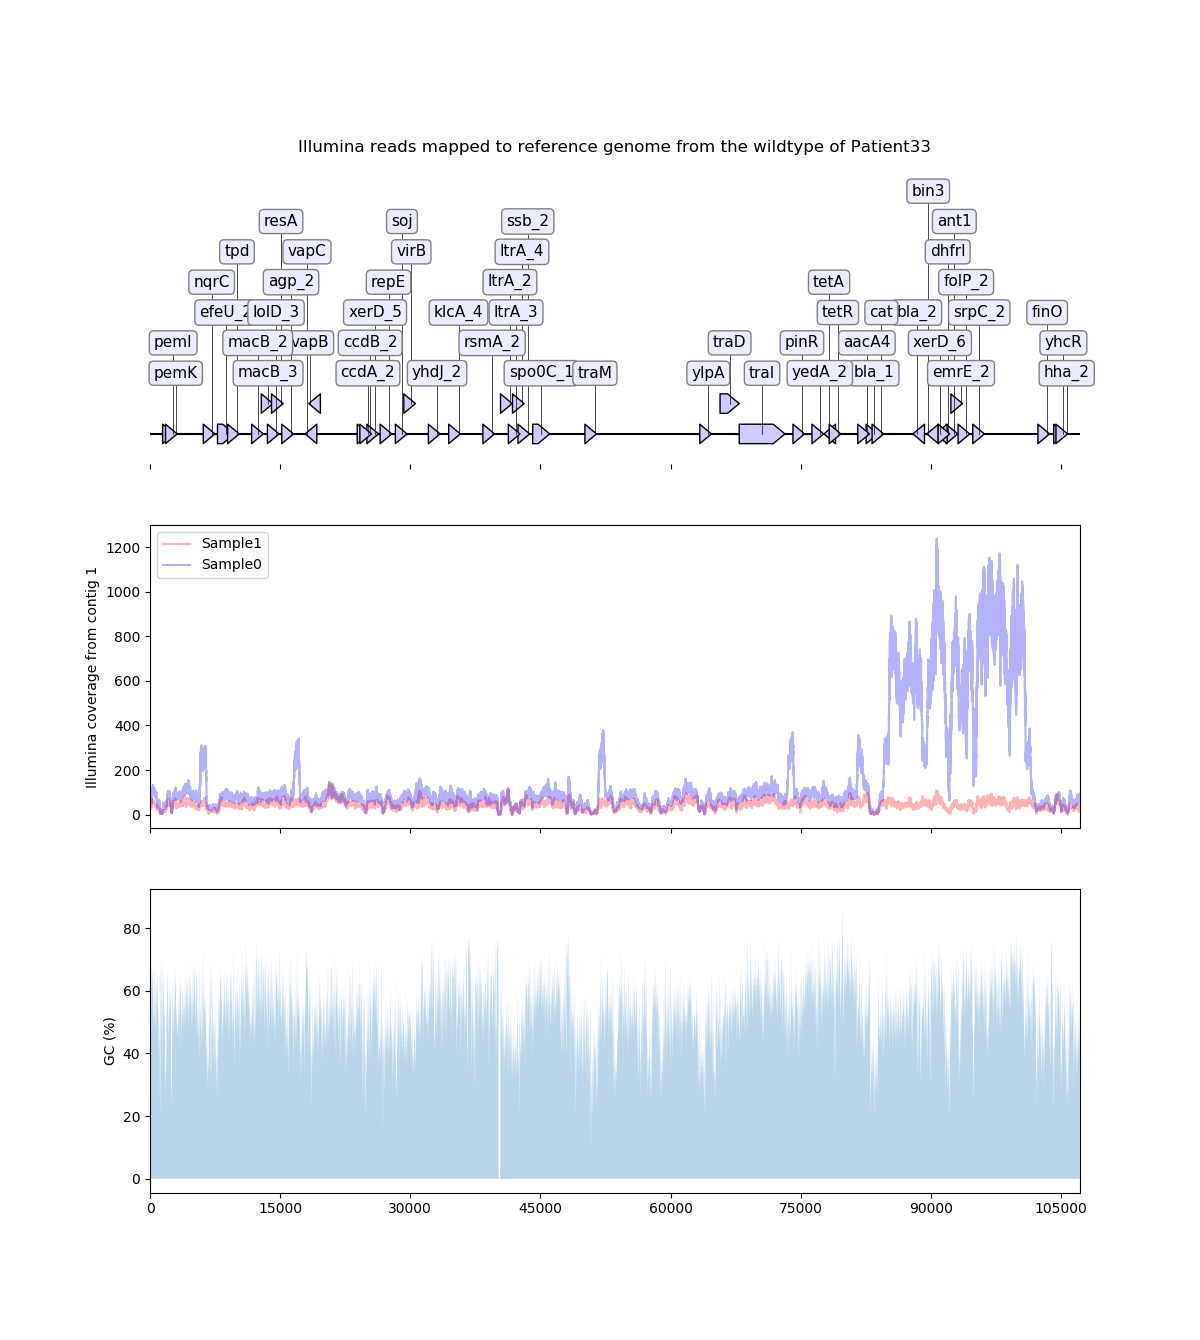
\includegraphics[scale=0.3]{coverage_pat33.png}
	\caption{Upper figure: Annotation of the whole plasmid. Middle figure: Coverage of the illumina sequencing data from sample 0 (resistant sample) and sample 1 (susceptible sample). Buttom figure: GC content.}
	\label{figure:coverage}
\end{figure}

\begin{figure}
	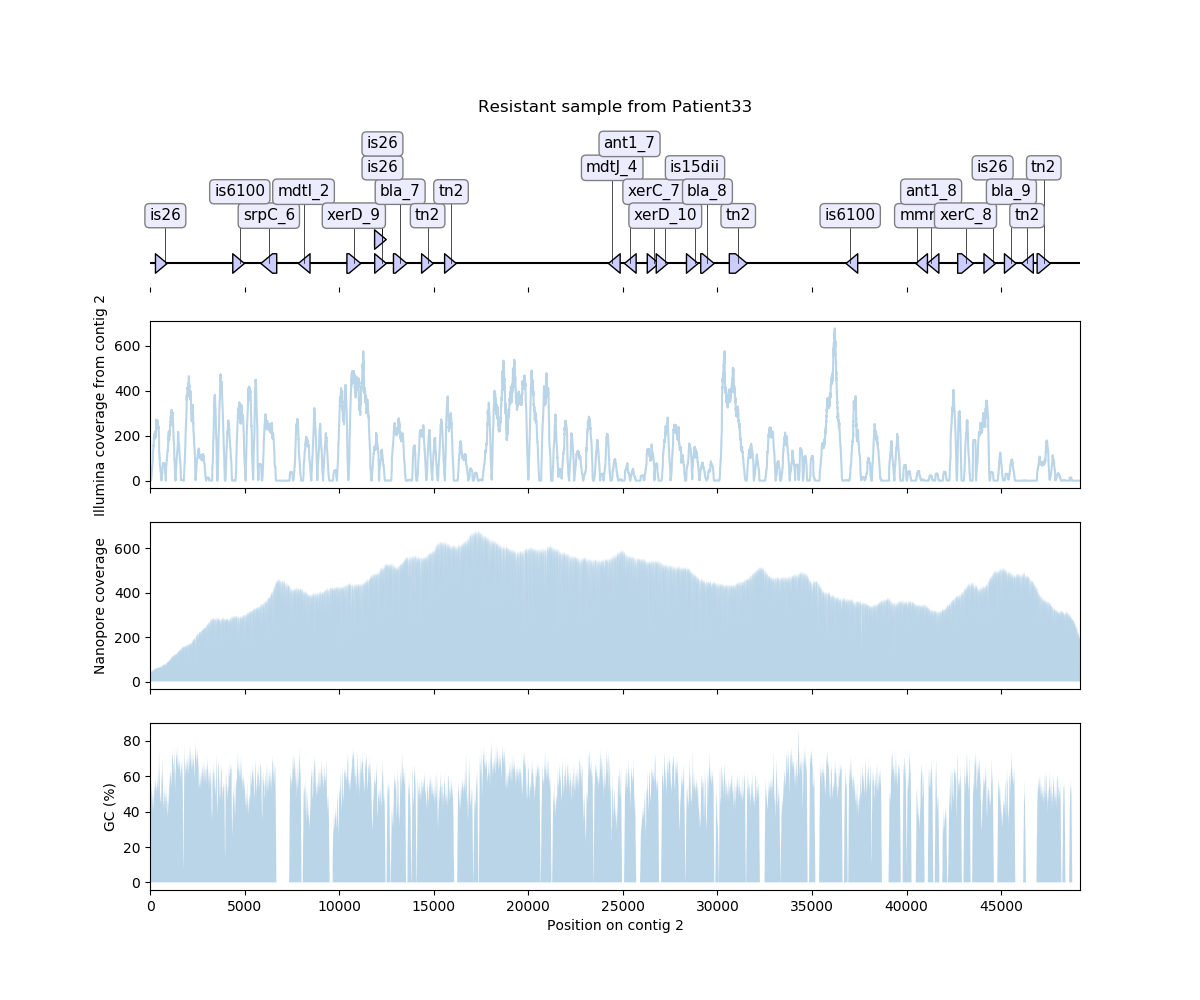
\includegraphics[width=0.5\textwidth]{sample0_plasmid.png}
	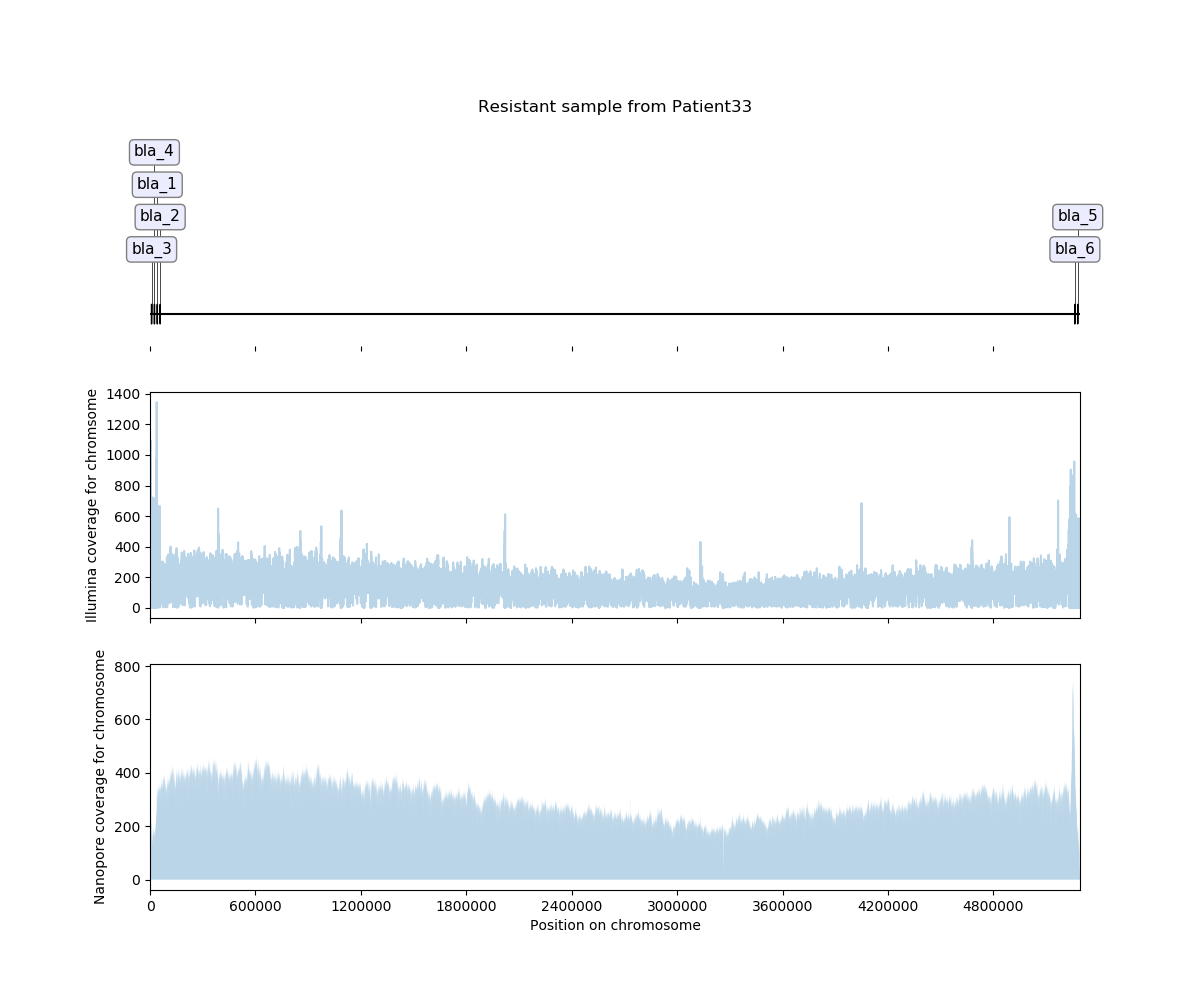
\includegraphics[width=0.5\textwidth]{sample0_chrom.png}
	\caption{}
\end{figure}
	
\subsection{Comparing ESBL genes in the resistant samples and the susceptible samples}
Since we long-read sequenced every sample from Table \ref{table:samples_overview} we hybrid-assembled and annotated those samples as well. This allowed us to see what ESBL genes were present in the susceptible and the resistant samples. The present ESBL genes and their copy numers are shown in Figure \ref{figure:esbl_genes}. Except for patient 33 there was no significant change in the copy numbers. But interestingly many strains lost or took up new ESBL genes over time. 
\begin{figure}[H]
	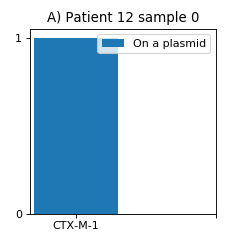
\includegraphics[width=.25\textwidth]{pat12s0.png}
	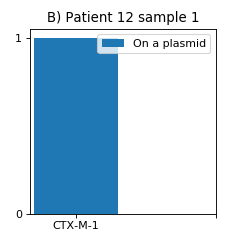
\includegraphics[width=.25\textwidth]{pat12s1.png}	
	
	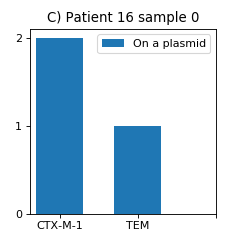
\includegraphics[width=.25\textwidth]{pat16s0.png}
	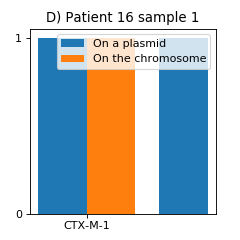
\includegraphics[width=.25\textwidth]{pat16s1.png}
	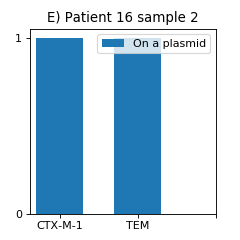
\includegraphics[width=.25\textwidth]{pat16s2.png}
	
	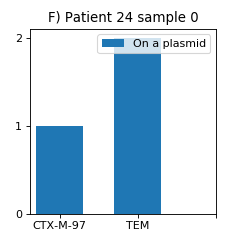
\includegraphics[width=.25\textwidth]{pat24s0.png}
	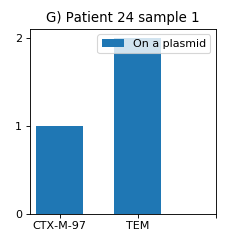
\includegraphics[width=.25\textwidth]{pat24s1.png}
	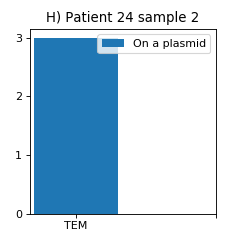
\includegraphics[width=.25\textwidth]{pat24s2.png}
	
	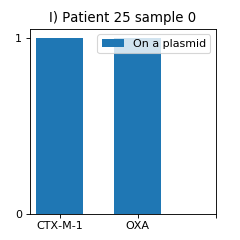
\includegraphics[width=.25\textwidth]{pat25s0.png}\hfill	
	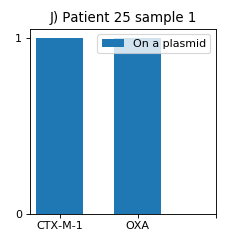
\includegraphics[width=.25\textwidth]{pat25s1.png}\hfill
	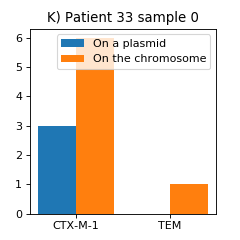
\includegraphics[width=.25\textwidth]{pat33s0.png}\hfill
	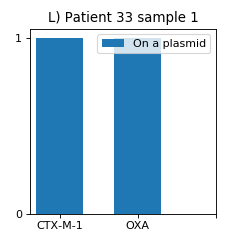
\includegraphics[width=.25\textwidth]{pat33s1.png}\hfill

	\caption{Copy numbers of ESBL genes. A-B: Patient 12, sample 1 resistant. C-E: Patient 16, sample 1 and 2 resistant. Change of copy number of CTX-M-1 and TEM. F-H: Patient 24, sample 1 resistant. CTX-M-97 was lost over time, increase of TEM copy number. I-J: Patient 25, sample 0 resistant. K-L: Patient 33 sample - resistant. Resistant sample has 8 more copies of CTX-M-1 where most of the copies are located on the chromosome.}
	\label{figure:esbl_genes}
\end{figure}

\section{Morbidostat experiments}
\subsection{Testing the continuous experiment}
The MIC of amoxicillin was determined as 2000 ng/\textmu l. The grow curve which was recorded before the initial experiment is shown in Figure \ref{figure:grow_curve}. It's visible that the growth slows down at an OD of 0.3, which is because 10 fold diluted media was used. 
\begin{figure}
	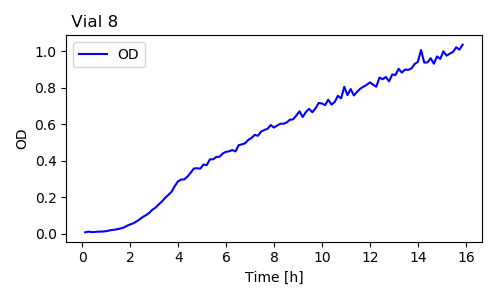
\includegraphics[width=.5\textwidth]{grow_curth.png}\hfill
	\caption{Grow curve of XL1 blue E. coli with 10 fold diluted LB media}
	\label{figure:grow_curve}
\end{figure}
The ODs and amoxicillin concentrations for the continous morbidostat experiment are shown in Figure \ref{figure:continuos_test}. Measuring of the OD for vial 1 behaved weirdly for the first 10 hours. This was caused by wrong calibration of the OD measuring unit, causing problems of detecting the right OD at low ODs. At around 40 hours 200 \textmu l of every cell susepension was transferred into 18 ml of new diluted media. It's visible that the accuracy of the OD measurement decreased before this dilution. That's because many dead cells caused scattering of the light which falsifies the OD measurement. In the second half of the experiment the drug concentrations were very high. Somehow the high amoxicillin concentration led to milky suspension when injected to the vials. This explanis why the OD measurements were more fuzzy towards the end. Also we observed that dead cells formed filament like aggregations. By stirring this sometimes caused wrong OD measurements as visible for vial 6 in Figure \ref{figure:continuos_test} at the end of the experiment. The morbidostat reacted very well to the detected growth of every vial. The target OD was set to 0.15 and every vial approximated this OD over time. Furthermore the algorithm reacted well by diluting with media when the cells died, or by increasing the drug concentration when the cells grew fast. \\
\begin{figure}
	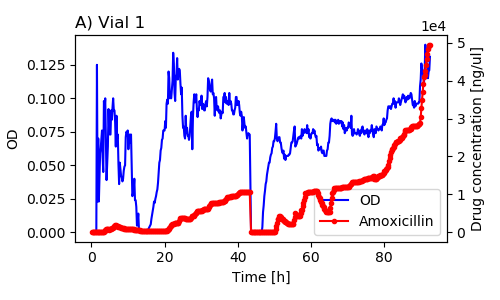
\includegraphics[width=.33\textwidth]{vial_1.png}\hfill
	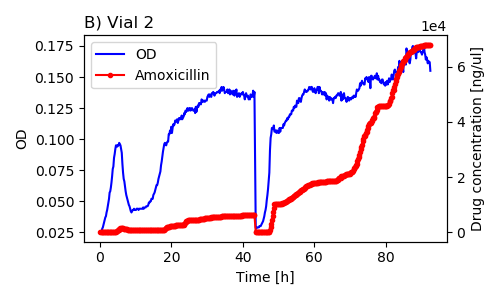
\includegraphics[width=.33\textwidth]{vial_2.png}\hfill
	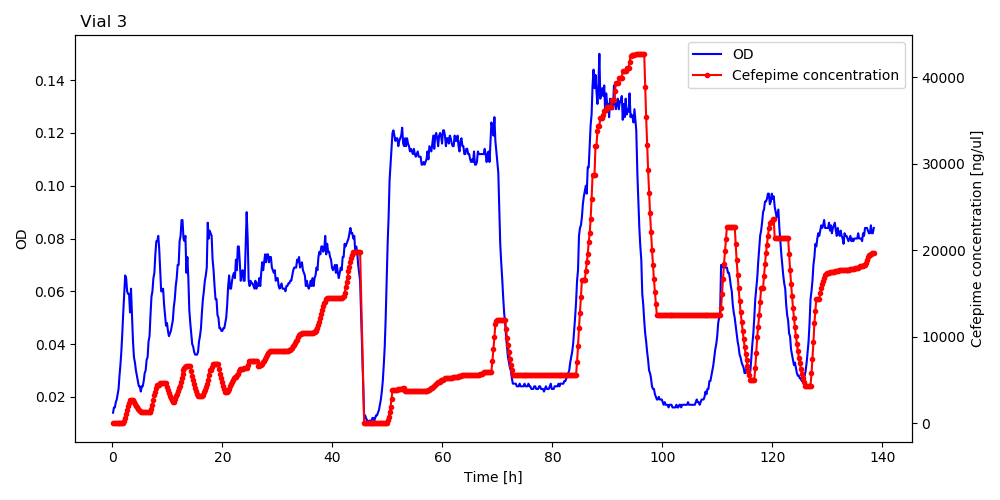
\includegraphics[width=.33\textwidth]{vial_3.png}\hfill
	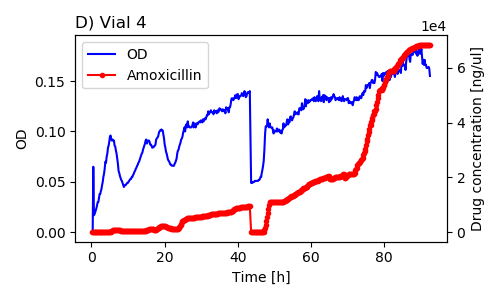
\includegraphics[width=.33\textwidth]{vial_4.png}\hfill
	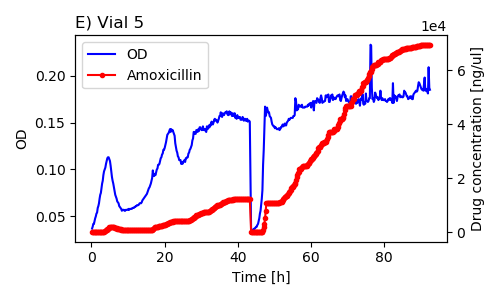
\includegraphics[width=.33\textwidth]{vial_5.png}\hfill
	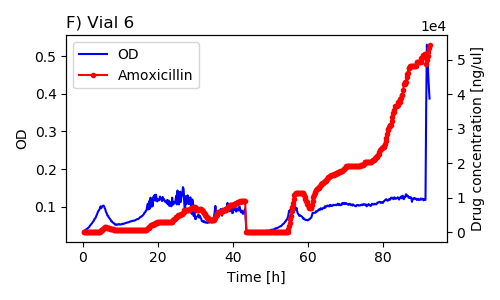
\includegraphics[width=.33\textwidth]{vial_6.png}\hfill
	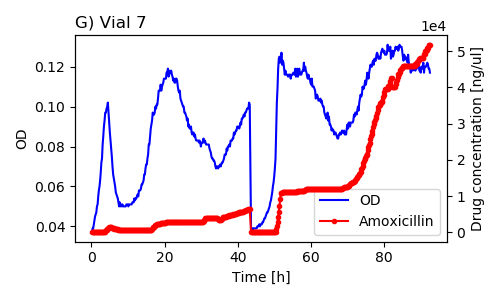
\includegraphics[width=.33\textwidth]{vial_7.png}\hfill
	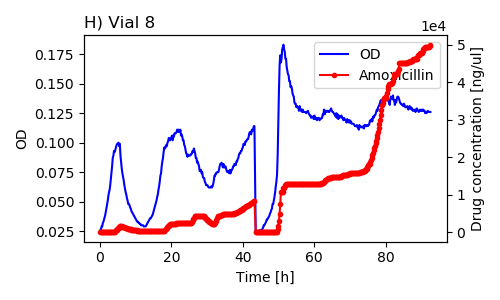
\includegraphics[width=.33\textwidth]{vial_8.png}\hfill
	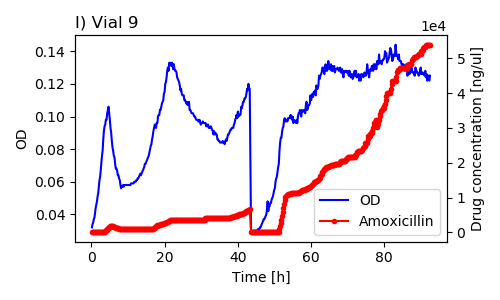
\includegraphics[width=.33\textwidth]{vial_9.png}\hfill
	\caption{For the continuous morbidstat experiment we cultured XL1 blue E. coli in 9 vials. Each plot shows the OD and the amoxicillin concentration for each vial over the whole experiment time (4.5 days). Dilution factor was 0.94, cycle time 12 minutes and the target OD 0.15. The kink in the OD and drug concentrations at 42 hours comes from transferring 200 \textmu l into new diluted media.}
	\label{figure:continuos_test}
\end{figure}
To get a better idea how the feedback reacted the first 40 hours of vial 8 are shown enlarged in Figure \ref{figure:continuos_test}. In this Figure it's visbile that no drug was injected until the OD of the vial was higher than the the drug\_dilution\_threshold (0.7). After that the amoxicillin concentration was constantly increased until the cells started to die. At the point where the OD decreased the concentration was stored which was 2000 ng \textmu /ml which is the same value as the MIC determined before the experiment. While the cells were dying media was added until the concentration was a quarter of the concentration which was necessary to kill the cells. With the cells starting to grow again, the drug concentration was increased up to the point where the cells started to die again. As visible in the Figure \ref{figure:vial8_zoom} double of the MIC was necessary to kill the cells this time.  
\begin{figure}
	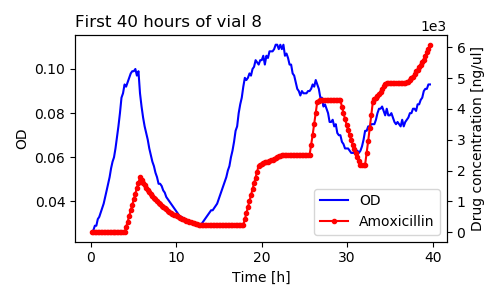
\includegraphics[width=.5\textwidth]{vial_8_zoom.png}
	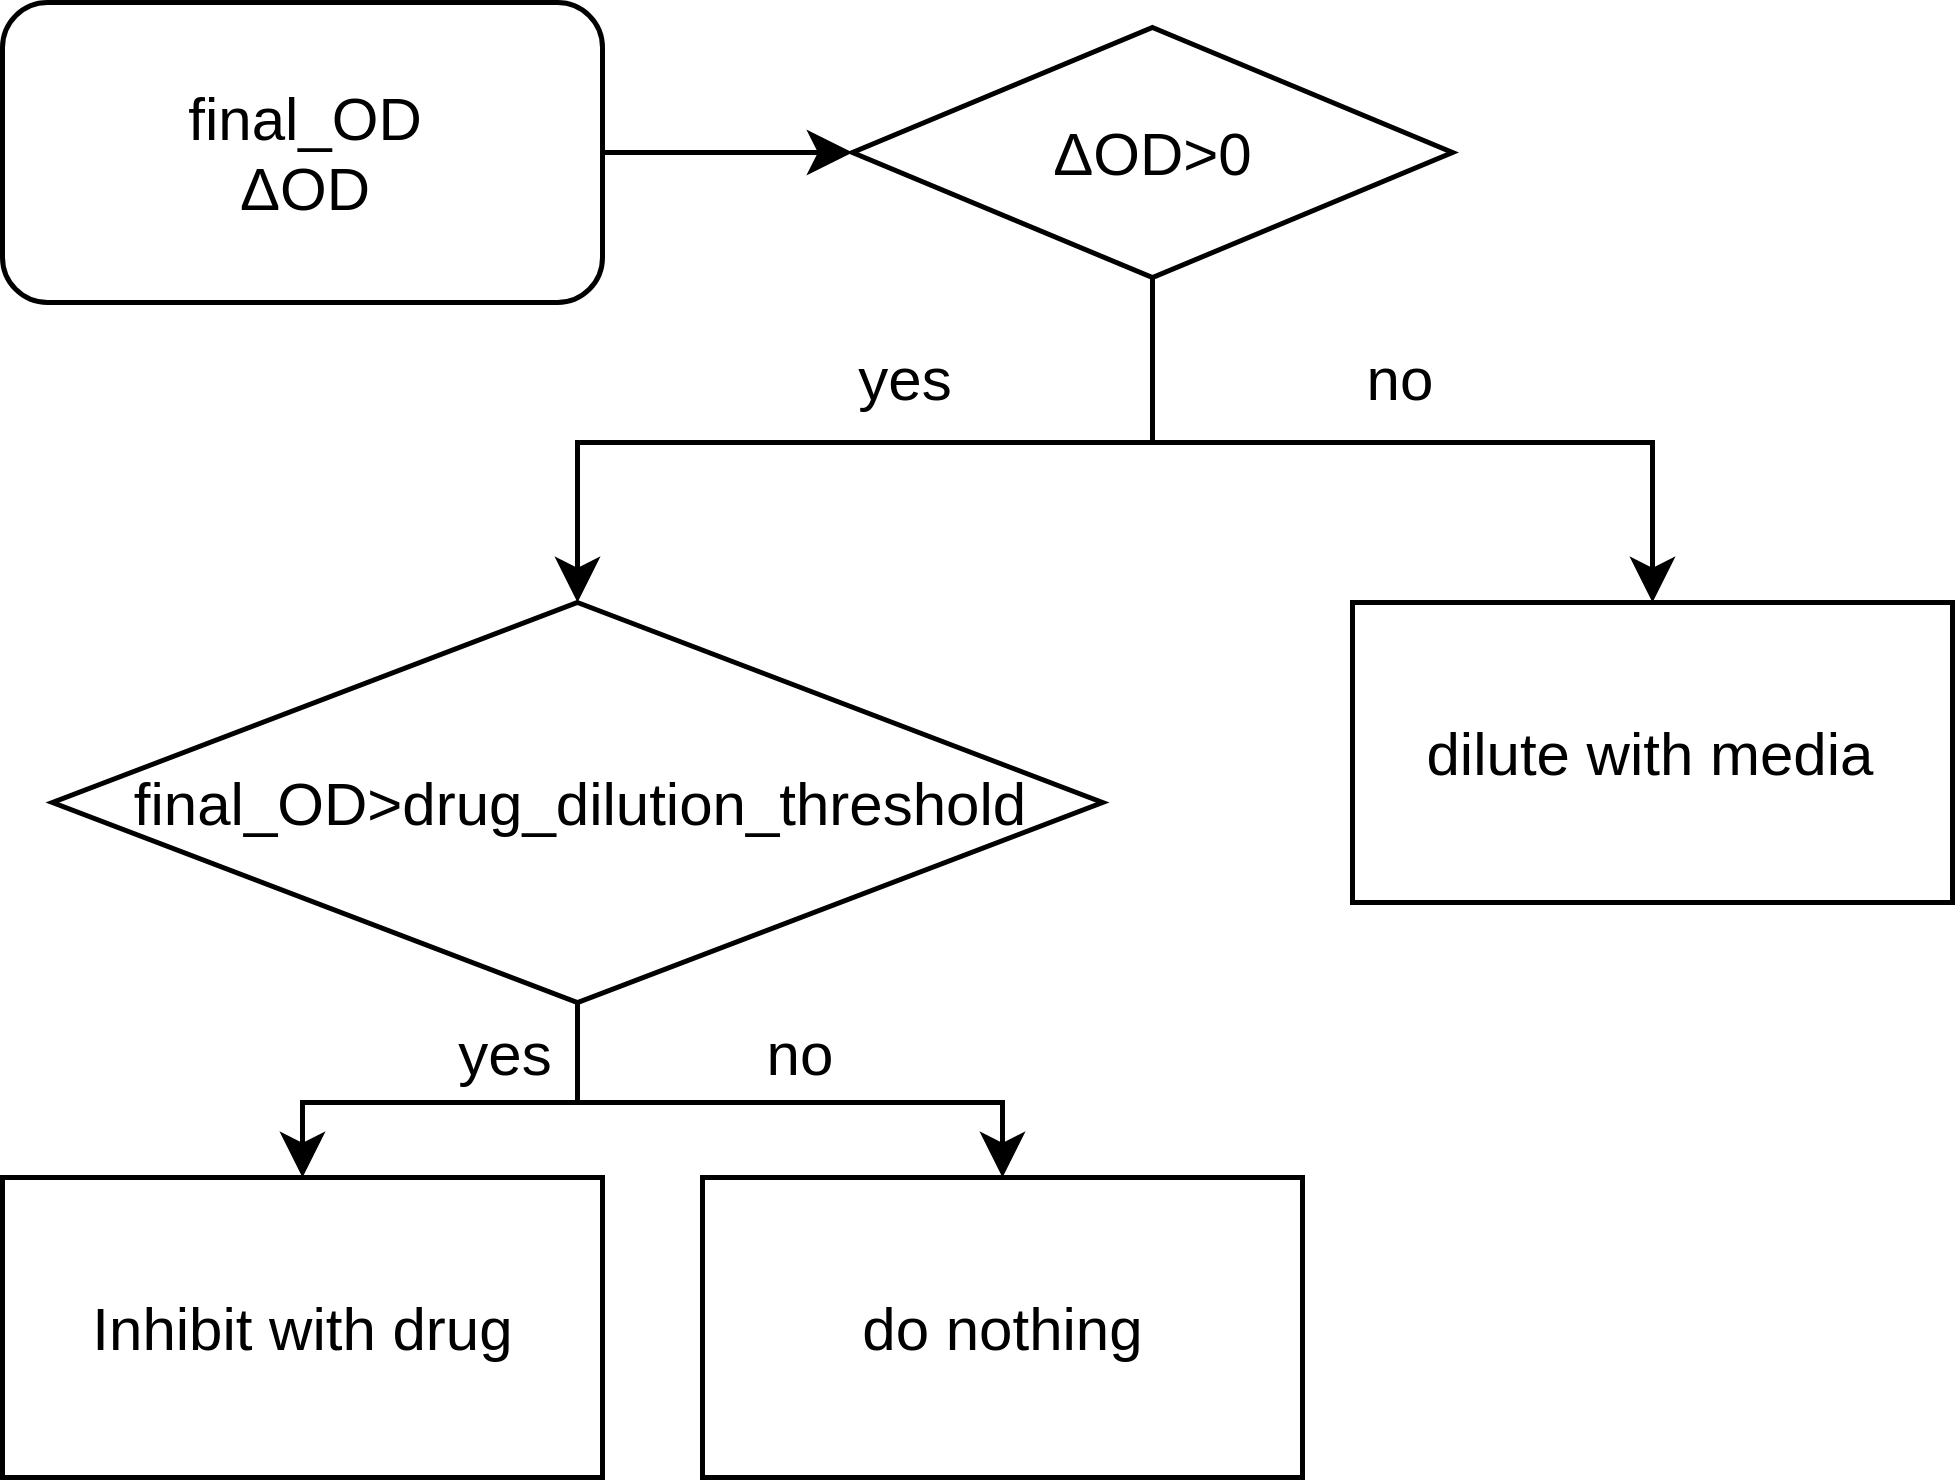
\includegraphics[width=.5\textwidth]{feedback.png}
	\caption{Left: First 40 hours of vial 8 from the continuous morbidostat. For the whole experiment time see Figure \ref{figure:continuos_test}. Right: Feedback algorithm deciding over drug injections. }
	\label{figure:vial8_zoom}
\end{figure}

\subsection{Morbidostat experiment 01}
\begin{figure}[H]
	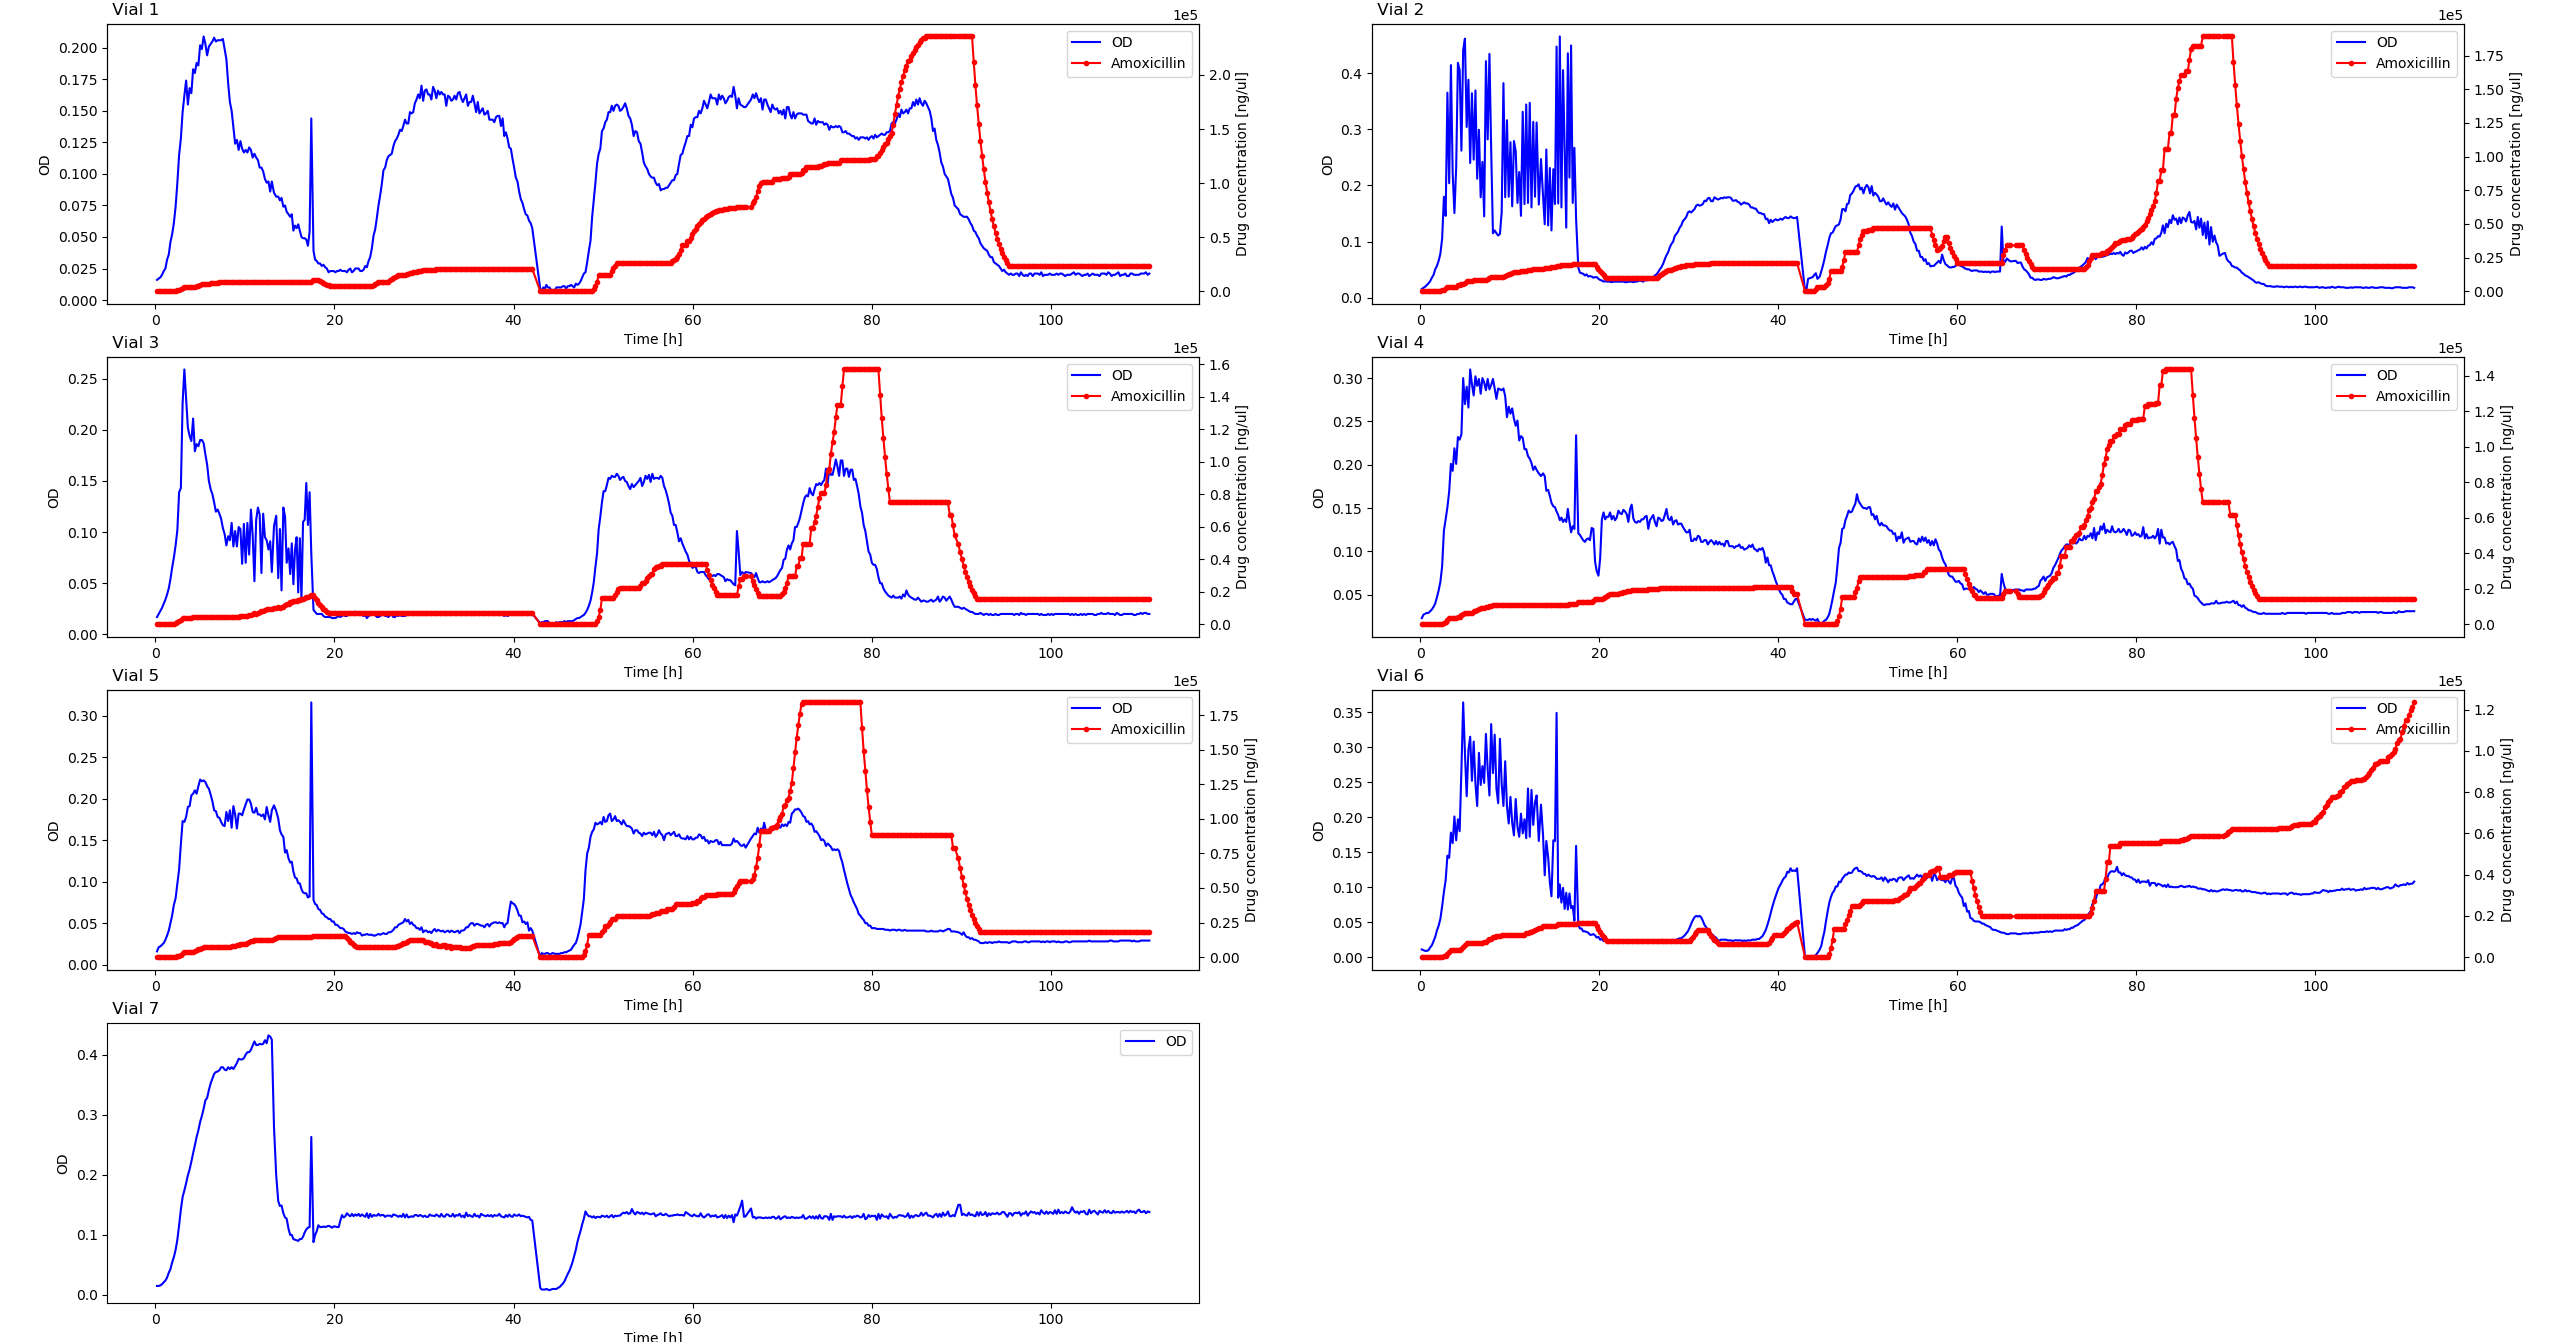
\includegraphics[width=1\textwidth]{01_morb_exp.png}
\end{figure}


\subsection{Morbidostat experiment 02}
\begin{figure}[H]
	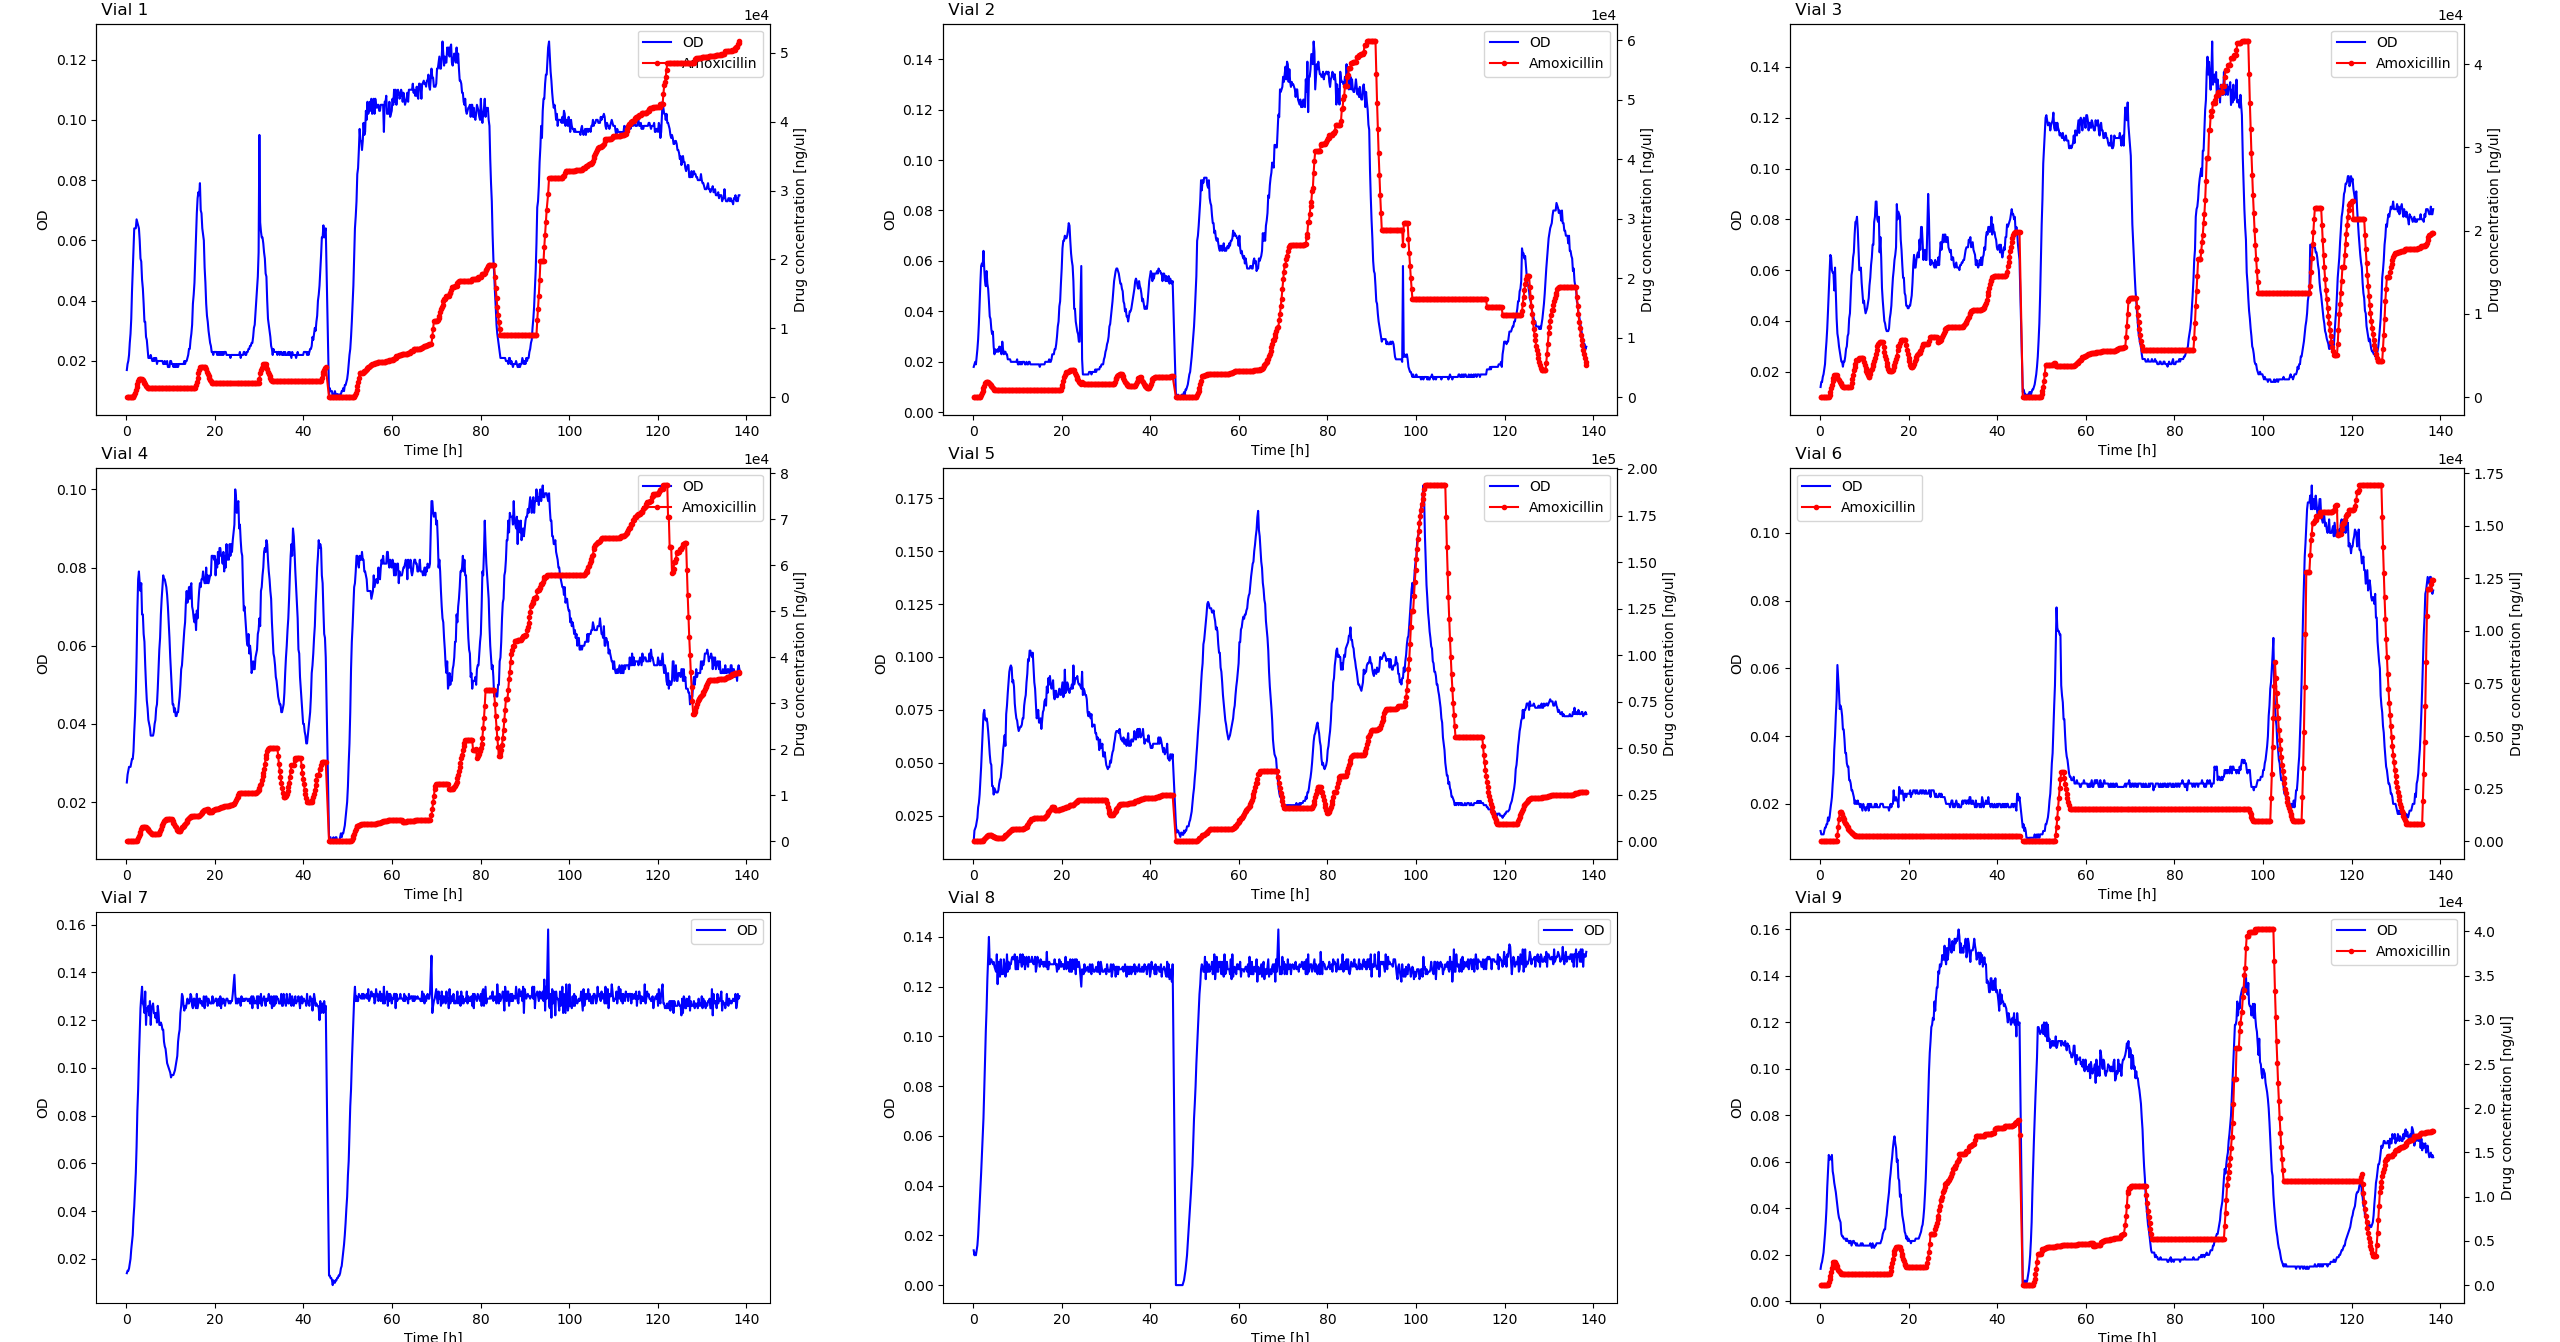
\includegraphics[width=1\textwidth]{02_morb_exp.png}
\end{figure}